\paragraph{Загрузка модели}

Первой функцией клиентской части является загрузка информационной модели,
прошедшей процесс упаковки (раздел~\ref{subsections:ServerImpl}).
Как говорилось ранее в разделе~\ref{subsections:ClientServerDesign},
в рамках прототипа реализована загрузка упакованной модели
с локального дискового устройства.

Для определения того, какие информационные модели прошли упаковку
и доступны для загрузки, необходимо сначала загрузить дополнительный AssetBundle,
автоматически создаваемый в процессе упаковки моделей
и называемый в фреймворке Unity манифестом ресурсных пакетов.
Этот AssetBundle содержит перечень всех пакетов, созданных во время экспорта.%
\cite{DocUnity,UnityAssetsResourcesBundles}
Загрузка манифеста будет осуществляться при инициализации загрузчика,
как это показано на рисунке~\ref{figure:SInitModelLoader}.

\begin{figure}[!htp]
    \centering
    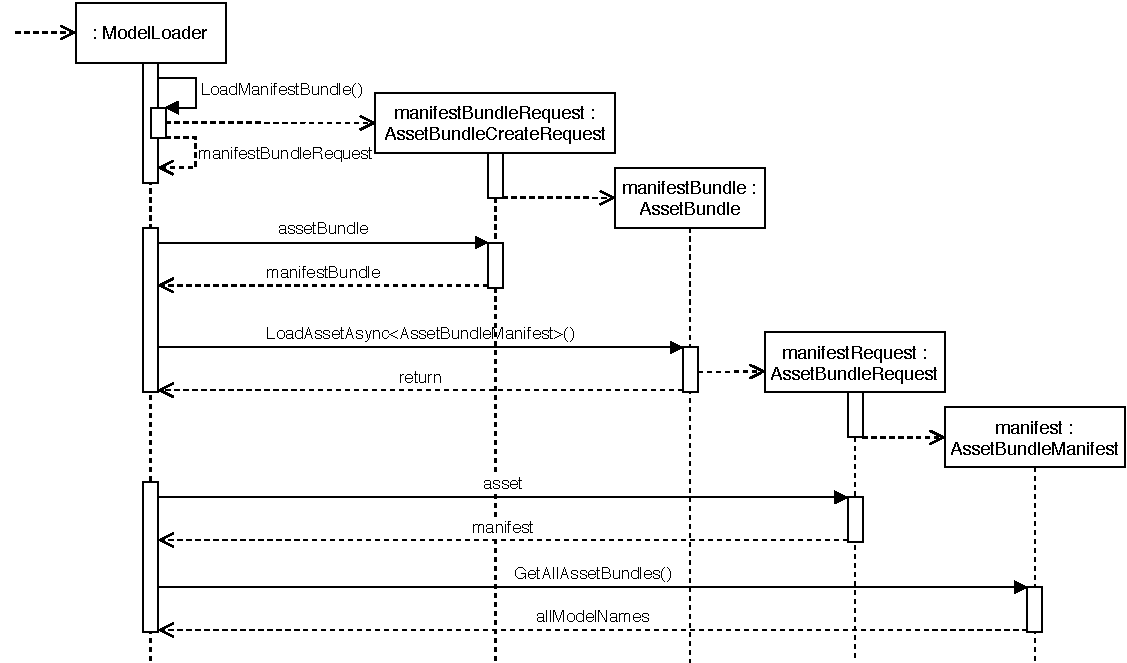
\includegraphics[width=1.0\textwidth]{images/UML-SInitModelLoader.pdf}
    \caption{Инициализация загрузчика моделей.}
    \label{figure:SInitModelLoader}
\end{figure}

Механизм инициализации загрузчика представляет собой асинхронную загрузку
ресурсного пакета, содержащего манифест, а за тем асинхронное его извлечение.
Процесс получение запроса пакета, содержащего манифест, не определен
в классе \emph{ModelLoader} и реализуется в его дочерних классах,
например на рисунке~\ref{figure:SLocalLoadManifestBundle} показана реализация
для локальной загрузки в классе \emph{LocalModelLoader}.

\begin{figure}[!htp]
    \centering
    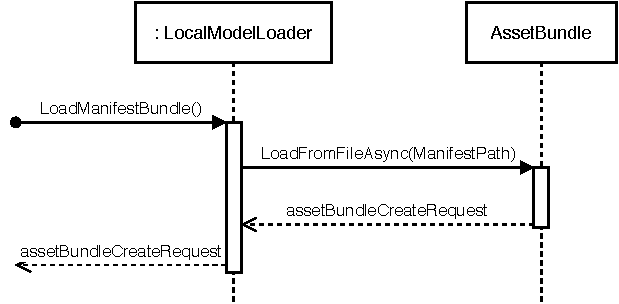
\includegraphics[width=0.7\textwidth]{images/UML-SLocalLoadManifestBundle.pdf}
    \caption{Загрузка локально-расположенного манифеста пакетов.}
    \label{figure:SLocalLoadManifestBundle}
\end{figure}

После инициализации загрузчик может принимать запросы моделей,
которые будет обрабатывать асинхронно, как изображено
на схеме~\ref{figure:SModelRequest}.
Загрузка ресурсного пакета с целевой информационной моделью аналогична тому,
как происходит загрузка манифеста: сначала происходит
асинхронная загрузка нужного ресурсного пакета,
а за тем асинхронное извлечение содержимого.
Процесс получения запроса нужного ресурсного пакета,
как и в случае с манифестом, не определен в классе \emph{ModelLoader},
а потому реализуется в дочернем классе,
как это показано на схеме~\ref{figure:SLocalLoadBundle}.
В отличие от загрузки манифеста теперь также требуется
отслеживать наличие уже загруженных информационных моделей (\emph{currentBundle})
для избежания перерасхода оперативной памяти.
Еще одним отличием выступает необходимость возврата загруженной модели
в асинхронном запросе, что реализовано через передачу в запрос
функции обратного вызова (\emph{onCompleteEvent}).

\begin{figure}[!htp]
    \centering
    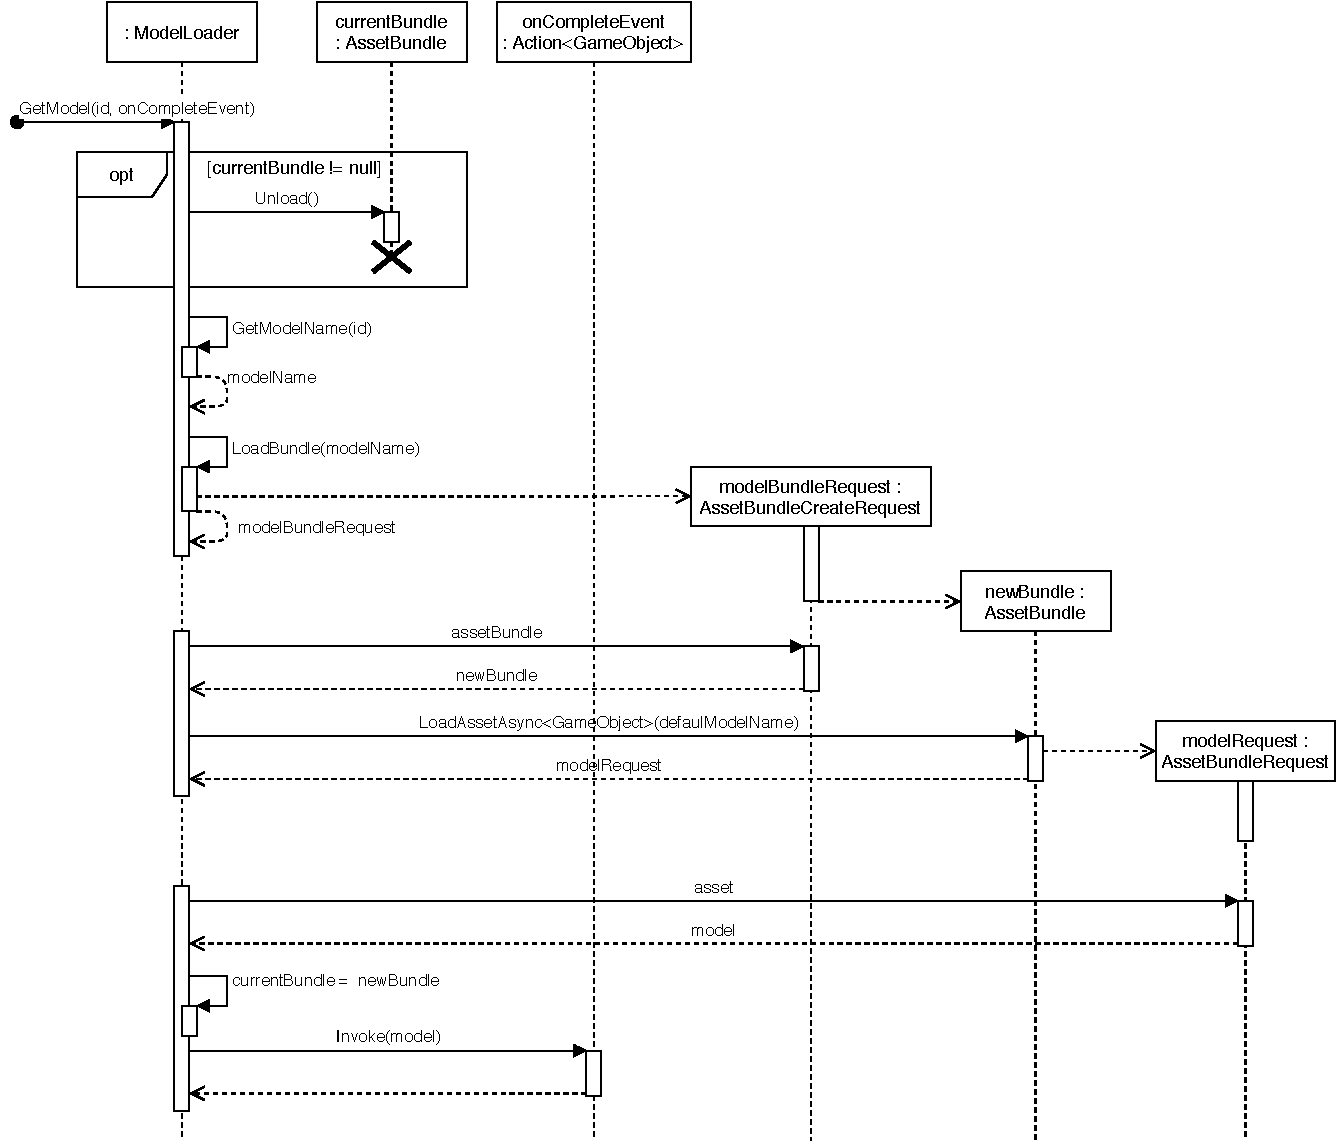
\includegraphics[width=1.0\textwidth]{images/UML-SModelRequest.pdf}
    \caption{Запрос загрузки модели.}
    \label{figure:SModelRequest}
\end{figure}

\begin{figure}[!htp]
    \centering
    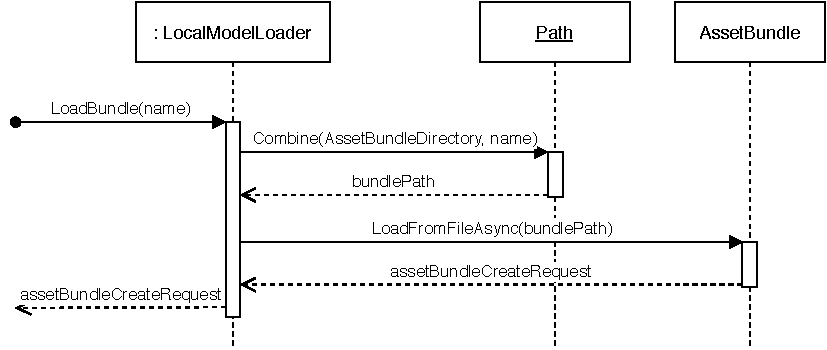
\includegraphics[width=0.8\textwidth]{images/UML-SLocalLoadBundle.pdf}
    \caption{Загрузка локально-расположенного ресурсного пакета.}
    \label{figure:SLocalLoadBundle}
\end{figure}
